\documentclass{beamer}

\usepackage{beamerthemesplit}
\usetheme{Singapore} 

\input{../../include/preamble.inc} 
\input{../../include/definitions.inc} 
\input{../../include/author.inc} 

\title[]{Введение в механику сплошных сред}

\begin{document}
	
\frame[plain]{\titlepage}

\frame[plain]{
	\frametitle{Аннотация}
	\parbox{\textwidth}{
		Предмет механики сплошных сред. Основные гипотезы механики сплошных сред. Понятие материальной точки. Лагранжево и эйлерово описание сплошной среды. Траектория, скорость, ускорение. Стационарное нестационарное течение. Линии тока поля скорости.
	}
}

\frame{
	\frametitle{Предмет механики сплошных сред}
	\begin{exampleblock}{}
		\alert{Механика сплошных сред} изучает движение газообразных, жидких и твёрдых деформируемых тел.
	\end{exampleblock}

\bigskip\bigskip\bigskip
\centering


\includegraphics[width=0.3\textwidth]{../img/tornado630.jpg}~
\includegraphics[width=0.3\textwidth]{../img/water-curl-wave-compressed.png}~
\includegraphics[width=0.3\textwidth]{../img/bone.jpg}


\bigskip
\tiny Л.И. Седов. Механика сплошной среды. Том 1. М.:Наука, 1970.
}

\frame{
	\frametitle{Разделы механики сплошных сред}
	
	\begin{itemize}
		\item Механика жидкости (гидродинамика, гидростатика)
		\item Аэрогазодинамика
		\item Механика деформируемого твердого тела (теория упругости, пластичности, разрушения)
		\item Механика плазмы
		\item Биомеханика
		\item Механика многофазных сред
	\end{itemize}
	
}

\frame{
	\frametitle{ Методы механики сплошной среды }

\begin{columns}
	\begin{column}{0.3\textwidth}
		\centering
		\alert{Дифференциальное исчисление}\\
		
	\bigskip
	Уравнения Эйлера:
	\begin{eqnarray*}
	\mathrm{div} \vec{v} & = &  0,\\	
	\frac{d\vec{v}}{dt} & = & -\frac{\nabla p}{\rho}.
	\end{eqnarray*}
	
	\end{column}
	\begin{column}{0.3\textwidth}
		\centering
		\alert{Интегральное исчисление}\\
		
		\bigskip
		Закон сохранения массы сплошной среды:
		
		\[
		\frac{\partial}{\partial t}\int\limits_{\omega_t}\rho d\omega = 0.
		\]
	\end{column}
	\begin{column}{0.3\textwidth}
	\centering
	\alert{Тензорный анализ}\\
	
	\bigskip
	Связь между тензором напряжения и тензором скоростей деформации для вязкой несжимаемой жидкости:
	
	\[
	\sigma = -p I + 2\mu \varepsilon.
	\]
\end{column}
\end{columns}	
	
	
}

\frame{
	\frametitle{ Основные гипотезы: евклидово пространство, время }
	
	\begin{exampleblock}{Евклидово пространство}
		\begin{itemize}
			\item Существует декартова система координат $(Oxyz)$
			\item Расстояние между точками $A$ и $B$ задаётся c мощью евклидовой метрики
			\[
			r_{AB} = \sqrt{(x_A-x_B)^2+(y_A-y_B)^2+(z_A-z_B)^2}
			\]
		\end{itemize}
		
	\end{exampleblock}

	\begin{exampleblock}{Абсолютное время}
		Время течёт одинаково во всех системах координат
	\end{exampleblock}
	
	\bigskip\tiny
	Нигматулин Р.И. Механика сплошной среды. Кинематика. Динамика. Термодинамика. Статистическая динамика. М.:ГЭОТАР-Медиа, 2014.
}

\frame{
	\frametitle{ Основные гипотезы: масса }
	
	\begin{exampleblock}{Абсолютная масса}
		\begin{itemize}
			\item У всех тел существует масса 
			\item Масса неотрицательна 
			\[
			m \geq 0
			\]
			\item Масса аддитивна 
			\[
			m_{A+B} = m_A+m_B
			\]
			\item Масса инварианта во всех системах координат, т.е. является скаляром
			
		\end{itemize}
		
	\end{exampleblock}
	
	\bigskip\tiny
	Нигматулин Р.И. Механика сплошной среды. Кинематика. Динамика. Термодинамика. Статистическая динамика. М.:ГЭОТАР-Медиа, 2014.
}


\frame{
	\frametitle{ Основные гипотезы: принцип равноправия инерциальных систем координат }
	
	\begin{exampleblock}{Постулат Галлилея}
		Формилировки всех физических законов не зависят от выбора инерциальной системы координат.		
	\end{exampleblock}
%	
%	\bigskip\tiny
%	Нигматулин Р.И. Механика сплошной среды. Кинематика. Динамика. Термодинамика. Статистическая динамика. М.:ГЭОТАР-Медиа, 2014.
}

\frame{
	\frametitle{ Основные гипотезы: принцип сплошности }
	\begin{exampleblock}{Определение}
	\parbox{\textwidth}{
	\alert{Сплошная среда} -- модель вещества, в которой распределение масса, сил, импульса, энергии и параметров, характеризующих состояние и движение этого вещества, определяется кусочно-непрерывными и дифференцируемыми функциями, заданными во всех точках рассматриваемого объема и во все моменты исследуемого времени. 	
	
%	\medskip
%	\tiny Эглит М.Э. Лекции по основам механики сплошных сред. Изд. 2-е, испр. М.: Книжный дом <<Либроком>>, 2010.		
	}	
	\end{exampleblock}




\begin{exampleblock}{Критерий сплошности}
\parbox{\textwidth}{
	
	Безразмерное \alert{число Кнудсена}
	\[
	\mathrm{Kn} = \frac{\lambda}{d} \ll 1,
	\]
	где $\lambda$ -- длина свободного пробега (в случае газа), расстояние между атомами, молекулами (жидкость, твердое вещество); $d$~--~характерный размер исследуемого явления. 
}

\end{exampleblock}


%		\bigskip\tiny
%	Нигматулин Р.И. Механика сплошной среды. Кинематика. Динамика. Термодинамика. Статистическая динамика. М.:ГЭОТАР-Медиа, 2014.
}


\frame{
	\frametitle{ Основные гипотезы: индивидуализация }
	
	\begin{exampleblock}{Приближение или гипотеза индивидуализации}
		Положение каждой точки, составляющей среду (континуум), можно находить в любой момент времени:
		\[
		\vec{r} = \vec{r}(t),
		\]
		\[
		\vec{r}_{t=0}= \vec{r}_0.
		\]
		
	\end{exampleblock}
	
%	\bigskip\tiny
%	Нигматулин Р.И. Механика сплошной среды. Кинематика. Динамика. Термодинамика. Статистическая динамика. М.:ГЭОТАР-Медиа, 2014.
}

\frame{
	\frametitle{ Основные гипотезы: средние величины }
	
	\centering
	\includegraphics[height=4cm]{../img/avg_area.pdf}~~~~~~~
	\includegraphics[height=4cm]{../img/avg_example.png}\\
{	\small
	Определение средней (макроскопической) плотности вещества, распределенного дискретно в пространстве
}	


	
	\begin{exampleblock}{Определение плотности и условие устойчивости}
	\[
		\tilde{\rho} = \frac{\delta m}{\delta V},\quad
		l_{micro} \ll \delta r \ll L.
	\]
	\end{exampleblock}
	
	
%	\[
%	\delta m = \sum_{i=1}^{\delta N}\mu^{(i)}
%	\]
	
	
%	\bigskip\tiny
%	Нигматулин Р.И. Механика сплошной среды. Кинематика. Динамика. Термодинамика. Статистическая динамика. М.:ГЭОТАР-Медиа, 2014}

}

\frame{
	\frametitle{ Материальная точка и поля в механике сплошных сред }
	\centering
	\begin{exampleblock}{Определение}
		\parbox{\textwidth}{
			\alert{Материальной точкой} или \alert{жидкой частицей} называется частица среды (вещества) как центра макроскопического объёма $\delta V$ с характерным размером порядка $\delta r$,  обладающий массой, импульсом, внутренней энергией и др., определяемыми в соответствии с условиями осреднения.
		}
	\end{exampleblock}

\begin{exampleblock}{Условия на поля, определяющие параметры тел}
	\begin{itemize}
		\item \textit{Устойчивость} (независимость от $\delta r$)
		\item \textit{Регулярность}  (непрерывность, дифференцируемость за исключением отдельных поверхностей, линий и точек)
		\item \textit{Представительность} (параметры тела являются интегралом от соответствующих параметров его составляющих жидких частиц)
	\end{itemize}
	
\end{exampleblock}

	
}


\frame{
	\frametitle{ Лагранжево описание сплошной среды }
	
	\begin{columns}
		\begin{column}{0.5\textwidth}
			\centering
			\includegraphics[width=\textwidth]{../img/lagranje.pdf}\\
			\small
			Перемещение и деформация сплошной среды при временах $0$, $t'$ и $t$, где 
			$\vec{r}_0 = \argxi$, $\vec{r} = \argx$
		
		\end{column}
		\begin{column}{0.5\textwidth}
			\centering
			Закон движения или \alert{траектории} материальных точек тела:
			\begin{eqnarray*}
				x_1 & =  & x_1\argtxi,\\
				x_2 & =  & x_2\argtxi,\\
				x_3 & =  & x_3\argtxi
			\end{eqnarray*}
		
		или
		\[
		\vec{r} = \vec{r}(t, \vec{r}_0).
		\]
			
		\end{column}
	\end{columns}


\begin{exampleblock}{Определение}
	\parbox{\textwidth}{
	Координаты материальных точек тела $\argxi$ называются \alert{лагранжевыми координатами} а такой подход \alert{лагранжевым}. 
}
\end{exampleblock}

	
}

\frame{
	\frametitle{ Принцип сплошности }
	
	\begin{exampleblock}{Критерий}
		Принцип сплошности реализуется, если 
		\[
		\Delta ^{(x,\xi)} = 
		\left|
		\begin{array}{ccc}
		\pd{x_1}{\xi_1} & 	\pd{x_1}{\xi_2} & 	\pd{x_1}{\xi_3} \\
		\pd{x_1}{\xi_2} & 	\pd{x_2}{\xi_2} & 	\pd{x_2}{\xi_3} \\
		\pd{x_1}{\xi_3} & 	\pd{x_3}{\xi_2} & 	\pd{x_3}{\xi_3} \\
		\end{array}
		\right| \neq 0.
		\]
	\end{exampleblock}

	\parbox{\textwidth}{
	Принцип сплошности \alert{нарушается} на ударных волнах, в зонах разрушения, разбрызгивания, при коагуляции капель, столкновении тел, на поверхностных, линейных и точечных источниках и стоках.	
	}
	
	
}

\frame{
	\frametitle{ Скорость материальных точек }
		\begin{columns}
		\begin{column}{0.5\textwidth}
			\centering
			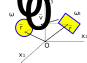
\includegraphics[width=\textwidth]{../img/velocity.pdf}\\
			\small
			Скорость точки вдоль траектории движения
			
		\end{column}
		\begin{column}{0.5\textwidth}
			\centering
		%	Закон движения или \alert{траектории} материальных точек тела:
			\begin{eqnarray*}
			v_1 & =  & v_1\argtxi,\\
			v_2 & =  & v_2\argtxi,\\
			v_3 & =  & v_3\argtxi
			\end{eqnarray*}
		
			или
			\[
			\vec{v}=\vec{v}(t,\vec{r}_0).
			\]
	
		\end{column}
	\end{columns}
	
	\begin{exampleblock}{Определение}
		\[
		\vec{v}(t, \vec{r}_0) = \lim_{\Delta t \to 0} \frac{\vec{r}(t+\Delta t, \vec{r}_0)-\vec{r}(t, \vec{r}_0)}{\Delta t} =
		\left. \pd{\vec{r}}{t} \right|_{ \vec{r} = \vec{r}_0 }.
		\]
	\end{exampleblock}
	
}


\frame{
	\frametitle{ Ускорение материальных точек }
	\begin{columns}
		\begin{column}{0.5\textwidth}
			\centering
			\includegraphics[width=\textwidth]{../img/accel.pdf}\\
			\small
			Ускорение материальной точки
			
		\end{column}
		\begin{column}{0.5\textwidth}
			\centering
			%	Закон движения или \alert{траектории} материальных точек тела:
			\begin{eqnarray*}
				a_1 & =  & a_1\argtxi,\\
				a_2 & =  & a_2\argtxi,\\
				a_3 & =  & a_3\argtxi
			\end{eqnarray*}
			или
			\[
			\vec{a}=\vec{a}(t,\vec{r}_0).
			\]
			
		\end{column}
	\end{columns}
	
	\begin{exampleblock}{Определение}
		\[
		\vec{a}(t, \vec{r}_0) = \lim_{\Delta t \to 0} \frac{\vec{v}(t+\Delta t, \vec{r}_0)-\vec{v}(t, \vec{r}_0)}{\Delta t} =
		\left. \pd{\vec{v}}{t} \right|_{ \vec{r} = \vec{r}_0 } =
		\left. \pdk{\vec{r}}{t} \right|_{ \vec{r} = \vec{r}_0 }.
		\]
	\end{exampleblock}
	
}

\frame{
	\frametitle{ Эйлерово описание сплошной среды}
		\begin{columns}
		\begin{column}{0.5\textwidth}
			\centering
			\includegraphics[width=\textwidth]{../img/euler.pdf}\\
			\small
			Перемещение и деформация сплошной среды при временах $0$, $t'$ и $t$, где 
			$\vec{r}_0 = \argxi$, $\vec{r} = \argx$
			
		\end{column}
		\begin{column}{0.5\textwidth}
			\centering
			
			Наблюдатель находится в точке $\argx$ и следит за изменением параметров среды со временем. 
			
		\end{column}
	\end{columns}
	
	
	\begin{exampleblock}{Определение}
		\parbox{\textwidth}{
			Координаты материальных точек тела $\argx$ называются \alert{эйлеровыми координатами} а такой подход \alert{эйлеров}. 
		}
	\end{exampleblock}
}

\frame{
	\frametitle{ Переход от лагранжевого представления к эйлерову }
	
	\parbox{\textwidth}{
	
	Пусть задан параметр среды $f$ в лагранжевых координатах
	\[
	f = f\argtxi.
	\]
	Если задан закон движения среды $\vec{r} = \vec{r}\argtxi$ и $\Delta^{(x,\xi)} \neq 0$, тогда 
	существует обратное преобразование:
	\begin{eqnarray*}
		\xi_1 & =  & \xi_1\argtx,\\
		\xi_2 & =  & \xi_2\argtx,\\
		\xi_3 & =  & \xi_3\argtx
	\end{eqnarray*}
	и 
	\[
	f\argtxi = f(t, \xi_1\argtx,  \xi_2\argtx, \xi_3\argtx) = 
	\]
	\[
		= \tilde{f}\argtx.
	\]
	}
}

	
	\frame{
		\frametitle{ Переход от эйлерова представления к лагранжеву }
		
		\parbox{\textwidth}{
			
			Пусть задан параметр среды $f$ в эйлеровых координатах
			\[
			f = f\argtx.
			\]
			Если задан закон движения среды $\vec{r} = \vec{r}\argtxi$, тогда 
%			существует обратное преобразование:
%			\begin{eqnarray*}
%				\xi_1 & =  & \xi_1\argtx,\\
%				\xi_2 & =  & \xi_2\argtx,\\
%				\xi_3 & =  & \xi_3\argtx
%			\end{eqnarray*}
%			и 
			\[
			f\argtx = f(t, x_1\argtxi,  x_2\argtxi, x_3\argtxi) = 
			\]
			\[
			= \bar{f}\argtxi.
			\]
		}
	}

\frame{
	\frametitle{ Стационарные движения и линии тока}
	\centering
	
	\begin{exampleblock}{Определение}
		\parbox{\textwidth}{
		Если при эйлеровом описании движение сплошной среды и её параметры не зависят от времени, а зависят только от от пространственных координат $\argx$, то такие движения называются \alert{установившимися} или \alert{стационарными}.
			
		}
				
	\end{exampleblock}

	\begin{exampleblock}{Определение}
		\parbox{\textwidth}{
			\alert{Линиями тока}, или \alert{векторными линиями} поля скорости $\vec{v}$, называются линии, касательные в каждой точке которых совпадают по направлению со скоростью $\vec{v}$ в этой точке в данный момент времени.
			
		}
		
	\end{exampleblock}
}
	
\frame{
	\frametitle{ Математическое описание линий тока }
	
	Уравнения линий тока
	\[
	d\vec{r} = \vec{v}\argx d\lambda,\quad (t=const),
	\]
	где $\lambda$ -- переменная, идентифицирующая точки вдоль линии тока. 
	
	Это уравнение сводится к 
	\[
	d\lambda = \frac{dx_1}{v_1\argtx} = \frac{dx_2}{v_2\argtx}= \frac{dx_3}{v_3\argtx},
	\]
	где $t$ является параметром и каждая линия тока относится к фиксированному моменту времени.
	
}
	
	
\frame{
	\frametitle{ Пример обтекания цилиндра}
	\centering
	

	\includegraphics[width=0.9\textwidth]{../img/stationary.png}\\
	\small Картины обтекания цилиндра набегающим потоком при различных числах Рейнольдса

	\bigskip
	\tiny
	\url{ http://www.heuristic.su/effects/catalog/est/byId/description/1201/index.html }
}

\frame{
	\frametitle{ Частная и субстанциональная (полная) производная }
	\centering


	Рассмотрим параметр среды, заданный в эйлеровых координатах $\varphi\argtx$ и закон движения сплошной среды $\vec{r}=\vec{r}\argtxi$.

	\bigskip
	\begin{exampleblock}{Частная производная в заданной точке пространства}
		\parbox{\textwidth}{
		
		$\displaystyle\pd{\varphi}{t}\argtx$ определяет изменение параметров в фиксированной точке пространства.
					
		}

		
	\end{exampleblock}


}

\frame{
	\frametitle{  Частная и субстанциональная (полная) производная }
		\begin{exampleblock}{Полная производная}
		\[
		\displaystyle\frac{d}{dt}\varphi(t, x_1\argtxi, x_2\argtxi, x_3\argtxi) = 
		\]
		\[
		=\pd{\varphi}{t}+\pd{\varphi}{x_1}\pd{x_1}{t}+\pd{\varphi}{x_2}\pd{x_2}{t}+\pd{\varphi}{x_3}\pd{x_3}{t}=
		\]
		\[
		= \pd{\varphi}{t} + \vec{v} \cdot \nabla \varphi = \left( \pd{}{t}+(\vec{v}\cdot \nabla) \right) \varphi
		\]
		\parbox{\textwidth}{
	
		определяет изменение параметра $\varphi$  в жидкой частице в фиксированной точке пространства, где
		$\vec{v}\argtx$ -- вектор скорости.
				
		}

		\end{exampleblock}

		\begin{exampleblock}{Определение}
			Оператор
	$
\displaystyle	\frac{d}{dt} =  \pd{}{t}+(\vec{v}\cdot \nabla)
	$
	называется оператором \alert{полной (субстанциональной)} производной.
	\end{exampleblock}

}


\frame{
	\frametitle{ Литература }
	\begin{itemize}[partopsep=1pt,label=\textbullet]
		\item {\em Л.И. Седов.} Механика сплошной среды. Том 1. М.:Наука, 1970.

		\item {\em Нигматулин Р.И.} Механика сплошной среды. Кинематика. Динамика. Термодинамика. Статистическая динамика. М.:ГЭОТАР-Медиа, 2014.
		
		\item {\em Эглит М.Э.} Лекции по основам механики сплошных сред. Изд. 2-е, испр. М.: Книжный дом <<Либроком>>, 2010.
		
	\end{itemize}
	
}


	
\end{document}
